\documentclass[a4paper]{article}

\usepackage{color}
\usepackage{graphicx}
\usepackage[normalem]{ulem}

\title{\textbf{Improved Vision and Scope Document and Interview Discussion}\\\large Requirements Engineering\\Group 42, SA: Tessa Schlief}

\author{Jos Vroegindeweij\\\texttt{s4776755} \and Wouter van Battum\\\texttt{s1011825}
\and Jaap Dijkstra\\\texttt{s4793048}}

\date{\today}

\begin{document}
\maketitle
\color{black}
\section{Product Vision and Business Requirements}
\subsection*{Business Requirements}
\subsubsection*{Background}
This project is about Seats and More. \color{blue}Seats and More started out as a single store with unique products with each its own story. It has now grown to a chain of 8 furniture stores, \color{black}with 8 physical stores in or near larger cities throughout the Netherlands. \color{blue} The aim is still to offer unique products in their stores. \color{black} The philosophy of Seats and More is that furniture should not be bought online: customers should be able to see, touch and test a chair, sofa, table or bed before deciding whether to buy it or not. \color{blue} The managers of the Seats and More store have been the only ones invested in the furniture chain from the opening of the store until now, no outside investors are involved. \color{black}

\subsubsection*{Business opportunities}
Seats and More has suggested an application that runs either on customers phones or phones available at the store that can navigate the customers through the store in a personalized manner while also recommending products to the customer, focusing on the products that they are interested in. This will allow clients to find the products they specifically are looking for faster and waste less time on products they are not interested in. Additionally, Seats and More suggested a product reviews system that customers can look at while shopping. \color{blue} This can help customers gain information about products more easily and make a better decision faster. \color{black}It was also suggested to potentially bring customers with similar interests in products together to further share their experiences on these products. This would allow customers to make a more weighted decision towards purchasing a product in the Seats and More store \color{blue}and could potentially help build a stronger clientele. \color{black}

\subsubsection*{Business Objectives}
The main ambition of Seats and More is to create a shopping experience that will please a growing group of returning customers. Seats and More hopes to attract both customers who still buy their furniture at physical stores as well as new customers who at this point are used to buying furniture online. The main objective is to have a 15\% increase in revenue after the first year after initial release. \sout{The other objectives are as follows:}
\begin{itemize}
\item \sout{Let the customers be navigated in a personalized manner through the store, focusing on the products that they are interested in, while avoiding congestions due to too many customers in a small area of the store.}
\item \sout{Let the customers be recommended products based on their interests. Should a particular product be sold out, an alternative product should be recommended to the customer.}
\item \sout{Provide the customers with product reviews or let them review a product themselves. These might be the reviews of all customers in the same physical store, or the reviews of all customers of all 8 physical stores.}
\item \sout{Let the customers create a wish list or shopping cart and then take the decision to buy the selected products via the website.}
\item \sout{BO-1: Attract 30 \% more old (customers that already used to come to the physical store) within 12 months.}
\item \sout{BO-2: Attract 50 \% new customers that used to shop for furniture online within 12 months.}
\item \sout{BO-3: Increase sales by 40 \% within 6 months.}
\end{itemize}

\subsubsection*{Success Metrics}
The success of the changes is measured by an increased number of satisfied customers, customers that have tested the furniture before buying it instead of only having seen a picture, \color{blue}and customers that have stated that the shopping experience is better than shopping online. \color{black}Seats and More also would like to see that these changes, as a result of an increased number of satisfied customers, result in less returned items.

\subsubsection*{Vision Statement}
For customers who want to buy furniture, the new product information system is an information system that will navigate the customers through the store in a personalized manner. The system also recommends the customers products based on their interests, and should a product be sold out, an alternative product should be recommended. This system should provide product reviews that the customers can read (or listen to) or provide themselves. The system should also have a wish list or shopping cart for customers to add selected products and make the decision to buy them via the website. Unlike the current way, where customers can buy furniture at online stores where the customers cannot see, touch, and test furniture, our product will create a shopping experience in physical stores that is as pleasant and personalized as possible.

\subsubsection*{Business Risks}
There are a few risks for Seats and More if they implement the new product information system. Due to software errors, Seats and More risk having congestions in the store. If the customers are not navigated the proper way, congestions can occur and that is what Seats and More wants to avoid. 
Seats and More risk having smart phones and/or tablets stolen. If customers pick up a smart phone or tablet at the entrance and do not return them, that could cost Seats and More a lot of money if it happens too often. 
Another risk is that customers do not want to come to a store and then have to buy their furniture online. 
Customers often tend to not want to put in too much effort, so they might lose customers over this.

\subsubsection*{Business Assumptions and Dependencies}
\begin{itemize}
\item Assumptions
\end{itemize}
Seats and More assumed that customers only want to see products that they are interested in, and not just look around in the store and see everything Seats and More has.
Seats and More assume that customers want to be recommended about other products.
They also assume that customers are willing to travel further distances to see the furniture, because eight stores throughout the Netherlands is not much.

\begin{itemize}
\item Dependencies
\end{itemize}
Seats and More is dependent on customers actually wanting to test and see the furniture they buy. Most web shops these days allow a customer to view a piece of furniture in the relevant room on their smartphone.
Seats and More is also dependent on the software engineers. If the software for the app is implemented wrongly, then for examples congestions can occur or customers could be sent to the wrong furniture in the store.

We have come to the conclusion that Seats and More is a company with big opportunities to grow and expand her clientele. Using this chapter, we are able to create the scope and limitations and business context of Seats and More.


\section{Scope and limitations}
\subsection*{Major features}
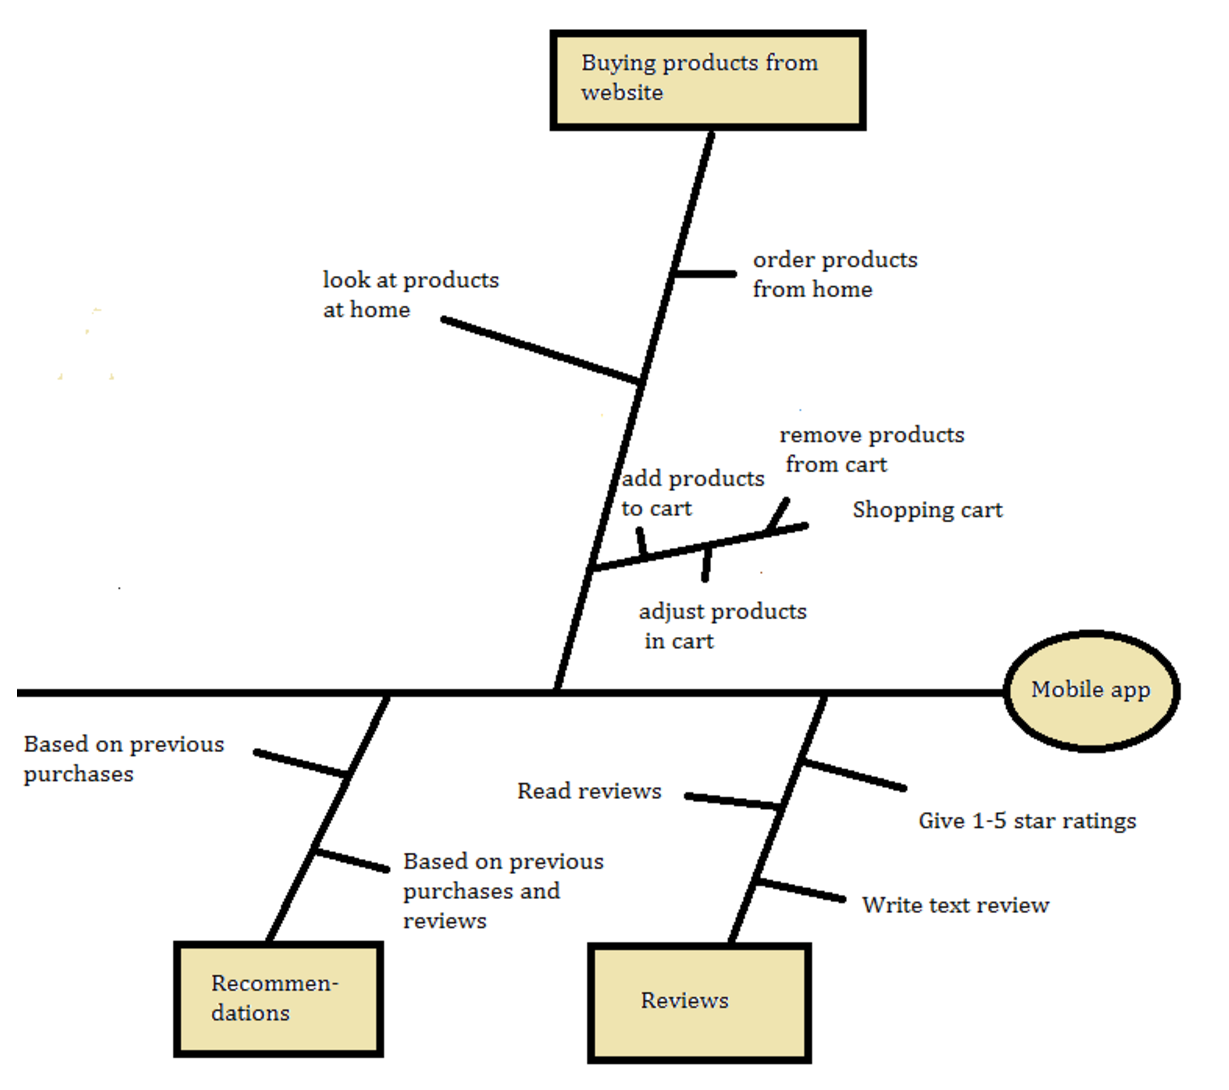
\includegraphics[scale=0.7]{new_feature_tree.eps}
\begin{itemize}
\item FE 1: \sout{Customers will be navigated through the store in a personalized manner, in such a way that there won't be congestions by having too many customers in the same area.}
\item FE 2: Writing and reading \sout{and listening to} product reviews
\item FE 3: Give recommendations to customers based on previous purchases and written reviews
\item FE 4: Placing products in shopping cart and buying them from a website at home.
\end{itemize}

Features that will \textbf{not} be implemented:
\begin{itemize}
\item \color{blue} Customers will be navigated through the store in a personalized manner, in such a way that there won't be congestions by having too many customers in the same area.

\item Customers can \textit{listen} to reviews.\color{black}

\item Bringing customers that are interested in the same products together to drink a cup of coffee.
\item Having the app integrated with in-store physical objects.
\end{itemize}

\subsection*{Scope of initial and subsequent releases}
\color{blue}As discussed with the management of \textit{Seats and More}, instead of having multiple subsequent releases, the focus will be entirely on the initial release of the system. The features implemented in this release will therefore be the major features discussed in the \textit{Major Features} section of this document.\color{black}
\subsection*{Limitations and exclusions}
\color{blue}The personalized route through the store is seen as less of a priority in the eyes of the management than the other major features and therefore will not be implemented.\\
\\
Listening to reviews has been rejected by the management because the management does not like seeing people walk around the store with headphones on.\\
\\
Bringing customers that are interested in the same products together to drink coffee will not be done as the majority of the management does not support the implementation of this feature.\\\color{black}
\\
Using in-store objects to communicate with the app is infeasible and will therefore not be implemented.

\section{Business Context}
\subsection*{Stakeholder profiles}
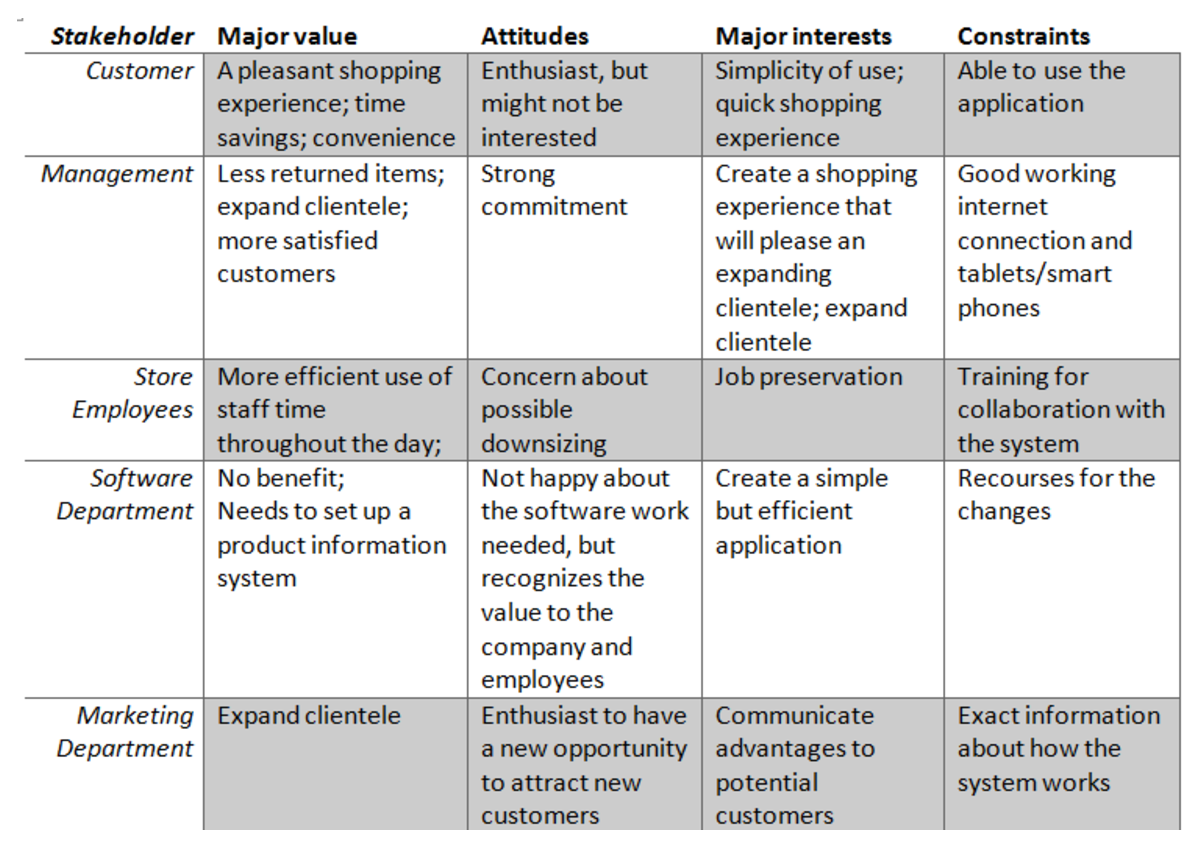
\includegraphics[scale=0.7]{stakeholder_profiles.eps}

\subsection*{Project priority}
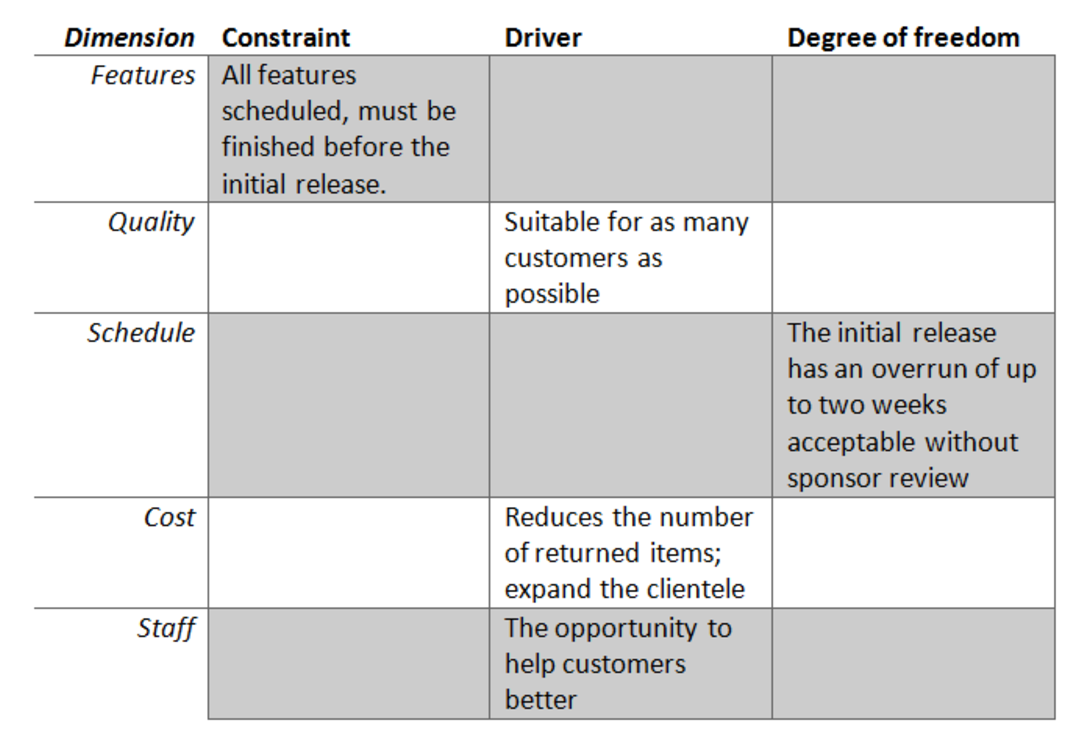
\includegraphics[scale=0.8]{project_priority.eps}

\subsection*{Deployment considerations}
The internet server must be upgraded to handle the increased usage of the internet by all the smartphones or tablets. The app has to be developed for different operating systems, such as iOS, Android or Windows Phone or tablet. Any infrastructure changes must be in place before the initial release. The customer database must have enough storage to store the preferences of the customers and the shopping cart. The store’s staff must get training to help them work with the new system in order to be able to help customers better.\\
\\
We have come to the conclusion that there are a lot of things to keep in mind and take into account when making the new product information system. 

\newpage

\section{Interview}
An overview of the complete questions and answers of the interview with the manager of \textit{Seats and More} can be found in Appendix A at the end of this document. Each question actively contributes to achieving the goals set out for the interview mentioned in the next paragraph. How exactly each question contributes towards the goals and helps us in finding the best implementation for the application is also included in Appendix A.

\subsection{Goals of the interview}
An important goal of the interview was to gain insight on the business objectives and success metrics according to \textit{Seats and More}. This would help us make sure that the project was going to be a success in the eyes of the most important stakeholder of the project, the management of \textit{Seats and More}. 

A second goal of the interview was to determine the audience that the management wishes the application to focus towards. If the target was older people for example, the implementation of the system would need to have a large focus on usability. If on the other hand the target audience would be younger people, the focus might learn more towards flexiblity of the application, shortcuts and quick responses from the application.

An other goal of the interview was to find out who the stakeholders were in this project. Knowing who to keep satisfied in the process of implementing the system is of course very useful information in succesfully developing and completing the project. Additionally, we wanted to find out the timeframe that is available for this project. Knowing the deadline for releasing the system is of course an integral part in keeping the stakeholders satisfied.

An other important aspect of the interview was finding out which of the suggested features had the biggest priority and which features had less priority according to the management. This information would help us make a judgment on implementing the system that best reflects the wishes of the management and at the same time is realistic for the available timeframe for the project.

\subsection{General implications}
From the interview we learned that there are no external parties involved in the \textit{Seats and More} furniture chain. This means that the most important stakeholders in this project are the Management and Marketing Department of \textit{Seats and More} and of course the customer.

\subsubsection*{User Requirements}

\paragraph*{Compared to persona's and stakeholders}
A user requirement that we recognized which relates to the customers as a stakeholder is a pleasant shopping experience. 

An other user requirement relates to the persona Michelle, 32 years old, who has limited time for shopping and does not want to be in the shop for too long. In her situation the product information next to the products could be a big help for her because she can quickly see the specifications. 

A user requirement that relates to Martha, who is 78 years old and does not have a smart phone, is the availability of the new system. With presenting smart phones or tablets at the entrance, this allows Martha to use the new system as well.

\paragraph{Compared to the business requirements}
The user requirements are aligned with the business objective of creating a shopping experience that will please a growing group of returning customers. With the implementation of the new system and presenting tablets or smart phones at the entrance of the store, we can also allow the elders who want to learn new things and the modern day technologies, to use the information system.

\paragraph{Compared to the scope}
A user requirement that is not aligned with the scope relates to the persona Michelle who does not have much time for shopping, so a personalized route through the store could help here. This function however will not be implemented in the new product information system.

\paragraph{Compared to the business context}
The user requirements are aligned with the business context, as stated in the deployment considerations, the application must be developed for multiple operating systems because then every customer can use the application.

The business context is also aligned with the user requirements because as stated in the stakeholder profiles, a major interest of the customers is that they want a quick shopping experience. From the persona Michelle, we get that she has limited time and therefore does not want to stay in the store for too long.

\subsection{Feature implications}
\subsubsection*{Reviews}
The interview has given us a lot of insight into which features have the highest priority in the project. For example, from the interview it became very clear that the Product Reviews were an integral part in the system to be designed. Providing reviews to the clients will help the users in making the best decision when shopping for furniture at \textit{Seats and More}.

\subsubsection*{Personalized route}
While in the initial Vision and Scope document our plan was to also implement the personalized route through the store, it  became clear that the priority for this feature was considerably lower than the other major features. This is why we have decided to not implement the personalized route through the store. 

\subsubsection*{Listening to reviews}
It also became clear that the management does not like seeing customers walk through the store with headphones on. We concluded from this that the feature that allows customers to listen to reviews using headphones should not be implemented, which we intented on doing initially. 

\subsubsection*{Available to everyone and easy-to-use}
The manager made it clear that the goal is to offer the services of the to be implemented system to both people that were proficient enough to use the app on their own mobile phone, as well as to customers that do not own a mobile phone or regularly use one. This means mobile phones or tablets should be present at the entrance to the store to be able to provide the service to these customers as well. An other important implication of this is that the application needs to be easy-to-use for everyone, as for example older people should be able to effectively use the application as well in order to get the best shopping experience.


\newpage
\section*{Appendix}
\appendix 
\section{Interview}
\textbf{Q}: Zou je wat meer kunnen vertellen over de achtergrond van Seats and More?
\textbf{A}: Degene die er mee begonnen is had eerst \'{e}\'{e}n winkel met redelijk unieke producten, waar overal een verhaal achter zat, dus geen standaard massa productie. Inmiddels uitgegroeid naar 8 filialen, inmiddels gebleken dat 8 filialen met unieke producten onmogelijk is, dus inmiddels wel veel dezelfde producten. Nog steeds wordt geprobeerd unieke producten aan te bieden.\\ 
\textit{This question helps us gain some insight on the background of \textit{Seats and More}, in particular how the \textit{Seats and More} organization was founded and how it has grown over time. }\\
\\
\textit{}
\textbf{Q}: Zijn er ook andere investeerders?\\
\textbf{A}: Nee, in principe alleen Seats and More zelf.\\
\textit{This question helps us understand who the stakeholders are in this project and thus who to keep satisfied when developing the system}\\
\\
\textbf{Q}: Wat zijn de doelen van het project? (Business Objectives?) \\
\textbf{A}: Natuurlijk meer omzet, over een jaar een groei van 15\% omzet kunnen zien.\\
\textit{This question helps us understand what the business objectives are of \textit{Seats and More}, and gives us more specific information on when the management would judge the project a success.}\\
\\
\textbf{Q}: Zijn er nog andere succes metrics?\\
\textbf{A}: Als klant zegt dat het een echte toevoeging is, en als klanten terugkomen omdat de ervaring beter is dan tegenover de website.\\
\textit{This again helps us understand what the objectives and success metrics of \textit{Seats and More} are. This helps us see how the management would judge the project a success.}\\
\\
\textbf{Q}: Hebben jullie in elke winkel hetzelfde assortiment?\\
\textbf{A}: Redelijk hetzelfde assortiment, af en toe zijn er producten die bij sommige winkels uitverkocht zijn maar in principe overal hetzelfde.\\
\textit{This question and the question below help us towards the goal of gaining some more background information on Seats and More, particularly about how the 8 physical stores work in terms of stock.}
\\
\textbf{Q}: Het is dus niet zo dat klanten naar verschillende winkels gaan omdat gedacht wordt dat er verschillende producten liggen?\\
\textbf{A}: In principe niet.\\
\\
\textbf{Q}: Kunt u de features raten in prioriteit?\\
\textbf{A}: De product informatie naast de producten zijn een grote prioriteit. De reviews zijn ook heel belangrijk, omdat mensen afgaan van wat andere mensen zeggen. Dus het kunnen zien en zelf schrijven van reviews is belangrijk. Het luisteren kan voor sommige mensen een leuke toevoeging zijn (Note: hier wordt later op teruggekomen!). Het algemene idee van mensen samen laten komen is dat dit niet nodig is. Producten in een wishlist plaatsen is natuurlijk wel nodig omdat mensen moeten kunnen bestellen. \\
\textit{This question contributes to the very important goal of finding out which features have the highest priority in the eyes of the management. This helps us judge which features to implement and which features not to implement so that the application best reflects the wishes of the management and at the same time is still realistic for the available timeframe.}\\
\\
\textbf{Q}: Hoe belangrijk is het om mensen thuis te kunnen laten betalen?\\
\textbf{A}: Dit is wel belangrijk omdat mensen vaak nog even na willen denken, en als ze dan weer speciaal terug naar de winkel zouden moeten is dat een extra drempel.\\
\textit{This question gives us information on the priority of this specific feature according to the management, as we had doubts about the priority and usefulness of this particular feature. }\\
\\
\textbf{Q}: Hoe belangrijk is de persoonlijke route door de winkel? Hoe ziet u het navigeren van mensen door de winkel voor zich, lampjes kunnen verwarrend zijn, kleuren misschien een oplossing?\\
\textbf{A}: Ik kan me dit inderdaad voorstellen, ik vind de reviews belangrijker dan de navigatie. Navigatie is wel interessant maar ook wel lastig omdat mensen vaak lekker zelf willen rondlopen. \\
\textit{This question gives us information about the priority of the navigation system itself, and also the relative importance of this feature compared to the other major features of the project.}\\
\\
\textbf{Q}: Hoe moet de navigatie er precies gaan uitzien? Is er een navigatie met een kaart?\\
\textbf{A}: Áls je de navigatie zou willen uitwerken dan zou ik wel zorgen dat mensen kunnen zien waar bepaalde producten liggen.\\
\textit{This gives us information on how the management would like the system to be implemented, which contributes towards the goal of determining when the management would deem the project a success.\\}
\\
\textbf{Q}: Hoe belangrijk is het voorkomen van ontstoppingen?\\
\textbf{A}: Wat mij betreft is dit niet zo belangrijk, omdat mensen dit uit zichzelf wel doen.\\
\textit{This question contributes towards the goal of determining the priority of avoiding congestions in the the store when using the personalized route. This helps us determine whether or not this aspect of the personalized route should be implemented.}\\
\\
\textbf{Q}: Is de voorkeur voor telefoons/tablets bij ingang van de winkel of een app op mobiel van klant?\\
\textbf{A}: Ik denk dat OOK op eigen telefoon ook leuk is, ik denk dat dat zeker wel mogelijk moet zijn. En als mensen zelf geen telefoon hebben, willen we ook zeker iets kunnen aanbieden om te gebruiken.\\
\textit{This question contributes to determining which part of the audience the management would like to focus their application on. This helps us determine the user values that need to be considered in the development of the system.}\\
\\
\textbf{Q}: De recommendations: bestaat er op dit moment al een soort klantenkaart systeem waarbij purchases worden bijgehouden waar we de recommendations initieel op kunnen baseren?\\
\textbf{A}: Nee dit bestaat nog niet.\\
\textit{This question and the question below help us understand how the to be implemented system should work, and thus tells us when the management would be satisfied with the developed system.}\\
\\
\textbf{Q}: We nemen aan dat het systeem alle 8 winkels samen moet nemen?\\
\textbf{A}: Ik denk dat we het initieel enkel in één winkel het hele systeem implementeren en vervolgens kijken of het interessant genoeg is om ook in de rest te implementeren.\\
\\
\textbf{Q}: Wanneer willen jullie het in gebruik nemen?\\
\textbf{A}: We willen het 1 september in gebruik nemen omdat eind september de drukke periode begint. Eind september is de laatst mogelijke deadline. Er zit dus maar 2-3 weken marge in, maar het liefst gewoon 1 september.\\
\textit{This question gives us information on when the management would like the system to be implemented ideally, and how much space there is for the release to be delayed if necessary. This helps us in planning the development of the system and of course tells us with which release date the management would be satisfied. }
\\
\textbf{Q}: De reviews moeten die van 8 winkels samen of individueel?\\
\textbf{A}: Hoe meer reviews hoe beter, dus uiteindelijk kunnen die allemaal samen. (Note: er werd genoemd dat eerst in één winkel het systeem geimplementeerd werd, dus waarschijnlijk in eerste instantie alle reviews ook gebaseerd op deze ene winkel?\\
\textit{This question and the question below also help us give information on how the management would like the application to be implemented.}\\
\\
\textbf{Q}: Is er een voorkeur tussen reviews ingesproken door klanten zelf of reviews die op worden gelezen d.m.v text to speech?\\
\textbf{A}: text to speech. Misschien is het luistergedeelte minder interessant.\\
\\
\textbf{Q}: Hoe ziet de review er precies uit? Iets met scores van 0 tot 5, een verhaaltje, pluspunten/minpunten noemen? \\
\textbf{A}: Voor de winkel is het interessant is een stukje tekst fijn. Maar het moet niet te uitgebreid worden, anders vullen mensen het niet in.\\
\\
\textbf{Q}: De alternative recommendations in het geval dat een product uitverkocht is, worden deze ook gebaseerd op interests van de specifieke klant of is dit gebaseerd op ideeën van de winkel zelf?\\
\textbf{A}: Winkel zelf.\\
\textit{This question and the two questions beow help us understand how specific features of the to be developed system should work, and thus gives us information on when the management would deem the system a success.}\\
\\
\textbf{Q}: Gebruikt de navigatie pijltjes om klanten te sturen of vertelt een stem waar de klant heen moet?\\
\textbf{A}: Ik denk dat het op beeld moet, niet perse met geluiden. \\
\\
\textbf{Q}: In het geval dat we al het systeem hebben om reviews te beluisteren, dan zou het een relatief simpele toevoeging zijn deze stem te implementeren.\\
\textbf{A}: Ik vind het niet zo'n leuk idee dat mensen met koptelefoons door de winkel lopen. Misschien is het luisteren naar reviews dan toch niet zo'n goed idee(!).\\
\textit{This question contributes towards the goal of determining the priority of the feature of allowing user to listen to reviews using headphones. This helps us decide whether or not this feature should be implented or not.}\\
\\
\textbf{Q}: De bedoeling was ook om de klantenkring uit te breiden, is er een bepaalde maatstaf die aangeeft of dit wel of niet gelukt is?\\
\textbf{A}: We hopen in ieder geval dat klanten aantallen niet terug lopen. We hopen op een stijging van 10-20\%.\\
\textit{This question contributes towards the goal of determining success metrics that we can strive towards in the development of the system. This gives us very specific information on how and when the management would deem the project a success.}

\end{document}
